% Beyond Density Matrices: Geometric Quantum States
% 	formerly:
% What is a Quantum State?
%
% fa: 4/31/20, 5/4/20, 7/15/20
% jpc: 5/1/20, 5/6/20, 7/19/20

%\documentclass[draft,nofootinbib,prl,twocolumn,showpacs,showkeys,groupaddress,preprintnumbers,floatfix]{revtex4-1}
\documentclass[draft,nofootinbib,pre,twocolumn,showpacs,showkeys,preprintnumbers,floatfix]{revtex4-1}

\usepackage{dynlearn}
\usepackage{graphicx}
\usepackage{physics}
\usepackage{multibib}
\newcites{SM}{SM References}
% \usepackage[utf8]{inputenc}
\usepackage{mathrsfs}
\usepackage[english]{babel}
\usepackage{amssymb,amscd}
\newtheorem{theorem}{Theorem}
\newtheorem{hypothesis}{Hypothesis}

% \newcommand{\norm}[1]{\left\Vert#1\right\Vert}
% \newcommand{\abs}[1]{\left\vert#1\right\vert}
% \newcommand{\set}[1]{\left\{#1\right\}}
% \newcommand{\R}{\mathbb{R}}
\newcommand{\e}{\mathrm{e}}
\newcommand{\Hilb}{\mathcal{H}}
\newcommand{\eps}{\varepsilon}
\newcommand{\To}{\longrightarrow}
\newcommand{\BX}{\mathbf{B}(X)}
\newcommand{\A}{\mathcal{A}}
\newcommand{\HH}{\Hilb}
\newcommand{\g}{\mathfrak{g}}
\newcommand{\Ug}{\mathcal{U}\mathfrak{g}}
\newcommand{\Tg}{\mathcal{T}\mathfrak{g}}
\newcommand{\Sg}{\mathcal{S}\mathfrak{g}}
\newcommand{\Us}{\mathcal{U}\mathfrak{s}}
\newcommand{\Ss}{\mathcal{S}\mathfrak{s}}
% \DeclareMathOperator{\Tr}{Tr}
\DeclareMathOperator*{\argmax}{arg\,max}
\DeclareMathOperator*{\argmin}{arg\,min}
\newcommand{\Ut}[1]{\undertilde{#1}}
\newcommand{\1}{\mathbbm{1}}
\newcommand{\circled}[1]{\tikz[baseline=(C.base)]\node[draw,circle,inner sep=1. 2pt,line width=0.2mm,](C) {\small #1};\!}
\newcommand{\Pexp}[1]{\mathrm{Pexp} \left[ #1 \right] }
\newcommand{\Ch}[1]{ \mathrm{Ch} \; #1}
\newcommand{\Sh}[1]{ \mathrm{Sh} \; #1}
% \newcommand{\Ket}[1]{ \left| #1 \right\rangle}
% \newcommand{\Bra}[1]{ \left\langle #1 \right|}
\newcommand{\Scal}[2]{ \left\langle #1 | #2 \right\rangle}
\newcommand{\KetQ}[1]{ \left| #1 \right]}
\newcommand{\BraQ}[1]{ \left[ #1 \right|}
\newcommand{\ScalQ}[2]{ \left[ #1 | #2 \right]}
\newcommand{\Miss}[2]{ \left[ #1 | #2 \right\rangle}
\newcommand{\MissQ}[2]{ \left\langle #1 | #2 \right]}
\newcommand{\ZT}{\undertilde{z}}
\newcommand{\Z}{\zeta}
\newcommand{\MV}[1]{\left\langle #1 \right\rangle}
\newcommand{\MC}[1]{\left\langle #1 \right\rangle_{\mathrm{mc}}}
% \newcommand{\braket}[2]{\langle #1 | #2 \rangle}
% \newcommand{\ketbra}[2]{| #2 \rangle\langle #1 |}
% \newcommand{\ket}[1]{| #1 \rangle}
% \newcommand{\bra}[1]{\langle #1 |}
\renewcommand{\equiv}{\coloneqq}
\newcommand{\PP}[4]{\mathbin{_{#2} P^{#1}_{#3}} \left[ #4 \right]}
\newcommand{\intP}{\int_{\mathcal{P}(\mathcal{H})} \!\!\!\!\!\!\!\!\!}
\newcommand{\intPB}{\int_{\mathcal{P}(\overline{\mathcal{H}})} \!\!\!\!\!\!\!\! \!}
\newcommand{\PH}{\mathcal{P}(\mathcal{H})}

\def\d{\delta}
\def\f{\frac}
\def\om{\omega}
\def\w{\wedge}
\def\la{\langle}
\def\ra{\rangle}
\newcommand{\p}{\partial}
\newcommand{\n}{\nabla}

\newcommand{\cg}[1]{{\color{blue}[[CG: #1]]}}
\newcommand{\fa}[1]{{\color{red}[[FA: #1]]}}
\newcommand{\cut}[1]{{\color{purple}[[CUT?: #1]]}}

\newenvironment{entry}
  {\begin{list}{--}{
      \setlength{\topsep}{0pt}
      \setlength{\itemsep}{0pt}
      \setlength{\parsep}{0pt}
      \setlength{\labelwidth}{5pt}
      \setlength{\itemindent}{0pt}}}{\end{list}}

\def\tbf #1 {\textbf{#1} }

\begin{document}

\def\ourTitle{%
% Interpretation of the Geometric Quantum State
% What is a Quantum State?
A kinetic theory of quantum information
}

\def\ourAbstract{%
TBD
}

\def\ourKeywords{%
Quantum Mechanics, Geometric Quantum Mechanics
}

\hypersetup{
  pdfauthor={Fabio Anza},
  pdftitle={\ourTitle},
  pdfsubject={\ourAbstract},
  pdfkeywords={\ourKeywords},
  pdfproducer={},
  pdfcreator={}
}

%%%%%%%%%%%%%%%%%%%%%%%%%%%%%%%%%%%%%%%%%%%%%%%%%%%%%%%%%%%%%%%%%%%%%%%%%%%%%%%

\title{\ourTitle}

\author{Fabio Anza}
\email{fanza@ucdavis.edu}

%\author{James P. Crutchfield}
%\email{chaos@ucdavis.edu}

\affiliation{Complexity Sciences Center and Physics Department,
University of California at Davis, One Shields Avenue, Davis, CA 95616}

\date{\today}
\bibliographystyle{unsrt}

\begin{abstract}
\ourAbstract
\end{abstract}

\keywords{\ourKeywords}

\pacs{
05.45.-a  %  Nonlinear dynamics and nonlinear dynamical systems
89.75.Kd  %  Complex Systems: Patterns
89.70.+c  %  Information science
05.45.Tp  %  Time series analysis
%02.50.Ey  %  Stochastic processes
%02.50.-r  %  Probability theory, stochastic processes, and statistics
%02.50.Ga  %  Markov processes
%%%%%%%FROM HERE%%%%%%
%05.20.-y  %  Classical statistical mechanics
%02.40.−k %Geometry, differential geometry, and topology
%03.65.−w %Quantum mechanics
%03.67.−a %Quantum information
%05.30.−d %Quantum statistical mechanics
%05.70.−a %Thermodynamics
%%%%%%%TO HERE%%%%%%
}

\preprint{\arxiv{2008.08682}}

\date{\today}
\maketitle

% \tableofcontents

% \setstretch{1.1}

% Collides with table of contents formatting
% \listoffixmes

% {\bf Lead Paragraph:
% }

\section*{Introduction.} The study of transport phenomena is crucial to harness 
the dynamical properties of natural systems. In this sense, transport theories are 
phenomenological descriptions of the nonequilibrium behavior of a system. Well-known 
examples are the theories of transport of charge, mass and heat. Most of them, were 
originally formulated to understand macroscopic phenomena like (in the case of 
mass transport) the tendency of a system to transfer mass in order to minimise the 
concentration difference. Over time, they were put on more rigorous ground using 
statistical mechanics and kinetic theory. Most notably, Boltzmann used this approach
to describe the behavior of gases, and explain the rise of macroscopic irreversibility from 
the underlying time-symmetric classical mechanics. After Boltzmann's work, the core idea 
of treating motion and interaction in a statistical way has led to innumerable advances, both 
of fundamental and applied nature. With the rise of quantum theory, these techniques have 
also been adapted to include quantum fluctuations, leading to improved descriptions of 
transport phenomena at the nanoscale.
While nowadays the use of kinetic and transport theories is ubiquitous, these techniques
have not been leveraged to study quantum information in closed and open quantum systems. 
Thus, in this work, we attempt to lay a bridge between the field of quantum information and 
that of transport theories. More accurately, here we provide a self-consistent theory to track
the dynamical evolution of a quantum state (and its probability distribution) in nonequilibrium
quantum systems. We do so by building a kinetic theory of quantum state evolution, on the quantum 
state space, both in closed and open configurations.

At the technical level, this is done by leveraging recent work \cite{Anza2020a,Anza2020b} on 
Geometric Quantum Mechanics: a differential-geometric approach to quantum mechanics that 
gets rid of the phase redundancy of the Hilbert space. The geometric formalism maps the Hilbert 
space onto a space of pure states that has the structure of a classical phase-space, with 
canonically conjugated coordinates.

The paper is organized as follows. In Section \ref{sec:GQM} we give a brief summary of 
GQM, and of the tools introduced in \cite{Anza2020a,Anza2020b}, both of which are needed.
In Section \ref{sec:IT} we give the first result: a microscopic derivation of the continuity equation 
for the information transport in quantum systems, with appropriate, microscopic definitions for 
phenomenological quantities such as fluxes and sink/sources terms. In Section \ref{sec:DYN}
we give the second result: a general equation of motion for the probability distribution that an open
quantum system is found in one of its quantum states. In Section \ref{sec:EXAMPLES} we provide
a few concrete examples, supported by numerical analysis. Eventually, in Section \ref{sec:FINAL}
we provide a quick summary and draw some conclusions.
 


%In the last fifty years we have witnessed an increasing use of
%information-theoretic techniques in virtually all scientific disciplines. Among all of them, the 
%cross-fertilization between physics and information theory has proven to be particularly fruitful.
%Within physics itself, it is hard to overstate the rise of quantum computing and quantum information 
%theory which, together with the modern experimental means to control nanoscale systems at the 
%level of individual components, has been addressed as a second quantum revolution \cite{Dow03}, 
%whose goal is to bring forth a new set of \emph{quantum technologies}. 
%While much work has been done to better understand the physical nature of information, when 
%compared to other fundamental concepts, such as the concept of energy, it is opinion of the author
%that our understanding is still very much at the 


%Within this larger perspective, in this work we address a single question: can we talk about information
%as a localized quantity, which moves around and can be exchanged?




\section{Geometric Quantum Mechanics}
\label{sec:GQM}

References
\cite{STROCCHI1966,Miel68,Kibble1979,Heslot1985,Page87,And90,Gibbons1992,Ashtekar1995,Ashtekar1999,Brody2001,Bengtsson2017,Carinena2007,Chruscinski2006,Marmo2010,Avron2020,Pastorello2015,Pastorello2015a,Pastorello2016,Clemente-Gallardo2013}
give a comprehensive introduction to GQM. Here, we briefly summarize only the
elements we need, working with Hilbert spaces $\mathcal{H}$ of finite dimension $D$.
For the details of the derivations, we send the reader to the literature cited above.

Given an arbitrary basis $\left\{\ket{e_n} \right\}_{n=0}^{D-1}$, a pure state is
parametrized by $D$ complex homogeneous coordinates $Z = \left\{      Z^n\right\}$, up to
normalization and an overall phase:
\begin{align*}
\ket{\psi} = \sum_{n=0}^{D-1} Z^n \ket{e_n}~.
\end{align*}
Here and throughout the paper we will always use upper indices to identify different 
coordinates of the same point and lower indices to identify different point. This 
description is redundant since we can renormalize $Z$ by multiplying it for a real number
and a phase (hence a complex number) and we would get the same physical situation. Therefore, 
$Z \in \mathbb{C}^{D}$, $Z \sim \lambda Z$, and $\lambda \in \mathbb{C}/\left\{ 0\right\}$. This equivalence 
relation means pure states of a quantum are points in the complex projective manifold $\mathcal{P}\left(
\mathcal{H} \right)=\mathbb{C}\mathrm{P}^{D-1}$. If the system consists of a single qubit, for
example, one can always use probability-phase coordinates $Z = (\sqrt{1-p},\sqrt{p} e^{i\nu})$.
We will often refer to this coordinates as they play a particular role.

\paragraph*{Observables and POVMs.} An \emph{observable} is a function $\mathcal{O}(Z) \in
\mathbb{R}$ that associates to each point  $Z \in \mathcal{P}(\mathcal{H})$ the
expectation value $\bra{\psi} \mathcal{O} \ket{\psi}/\braket{\psi}{\psi}$ of the corresponding
operator $\mathcal{O}$ on state $\ket{\psi}$ with coordinates $Z$:
\begin{align}
\mathcal{O}(Z) = \frac{\sum_{\alpha,\beta} \mathcal{O}_{\alpha,\beta}Z^\alpha \overline{Z}^\beta}{\sum_{\gamma} \left\vert Z^\gamma\right\vert^2}
  ~,
\label{eq:GQM_Observable}
\end{align}
where $\mathcal{O}_{\alpha \beta}$ is Hermitian $\mathcal{O}_{\beta,\alpha} = \overline{\mathcal{O}}_{\alpha,\beta}$.

Measurement outcome probabilities are determined by \emph{positive
operator-valued measurements} (POVMs) $\left\{E_j\right\}_{j=1}^D$ applied to a
state \cite{Nielsen2010,Heinosaari2012}. They are nonnegative operators
$E_j\geq 0$, called \emph{effects}, that sum up to the identity: $\sum_{j=1}^{D}
E_j = \mathbb{I}$. In GQM they consist of nonnegative real functions $E_j(Z)\ge
0$ on $\mathcal{P}(\mathcal{H})$ whose sum is always unity:
\begin{align}
E_j(Z) = \frac{\sum_{m,n}
  \left(E_j\right)_{m,n} Z^m \overline{Z}^n}{\sum_{k} \left\vert Z^k \right\vert^2}
  ~,
\label{eq:GQM_POVMs}
\end{align}
where $\sum_{j=1}^{D}E_j(Z) = 1$.

The quantum state space $\mathcal{P}(\mathcal{H})$ has a preferred metric 
$g_{FS}$---the \emph{Fubini-Study metric} \cite{Bengtsson2017}---and an 
associated volume element $dV_{FS}$ that is coordinate-independent and
invariant under unitary transformations. The geometric derivation of $dV_{FS}$
is beyond our immediate goals here. That said, it is sufficient to give its
explicit form in the probability-phase coordinate system $Z^n =
\sqrt{p_n}e^{i\nu_n}$ that we use for explicit calculations: 
\begin{align*}
dV_{FS}
  & = \sqrt{\det g_{FS}}
  \prod_{n=0}^{D-1} dZ^n d\overline{Z}^n \\
  & =  \prod_{n=1}^{D-1} \frac{dp_n d\nu_n}{2}
  ~.
\end{align*}
Notice how $p_0$ and $\nu_0$ are not involved. This is due to
$\mathcal{P}(\mathcal{H})$'s projective nature which guarantees that we can
choose a coordinate patch in which $p_0 = 1 - \sum_{n=1}^{D-1}p_n$
and $\nu_0 = 0$. As we will see now, these coordinates play a particular role:
they are canonically conjugated.

\paragraph*{State-space structure.} Beyond the Riemannian structures, it can 
be shown that $\PH$ also has another interesting geometric feature: a symplectic structure.
This is the hallmark of classical state spaces and justifies the use of the term 
\emph{quantum state space} for $\PH$. With a more common jargon, a symplectic
structure is the geometric entity allowing us to define ``Poisson Brackets''
and the existence of canonically conjugated coordinates. In particular, using 
probabilities and phases coordinates $\left\{ (p_n,\phi_n)\right\}$
one has that $\left\{ p_n , \phi_n \right\} = \frac{1}{\hbar}\delta_{nm}$. Thus,
for arbitrary functions $A$ and $B$ on $\PH$ one has
\begin{equation}
\left\{ A, B\right\} \coloneqq \frac{1}{\hbar}\sum_{n=1}^{D-1} \frac{\partial A}{\partial p_n} \frac{\partial B}{\partial \phi_n} - \frac{\partial B}{\partial p_n} \frac{\partial A}{\partial \phi_n}
\end{equation}


\paragraph*{Unitary evolution.} In QM, an isolated quantum system evolves
with a unitary propagator $U(t,t_0) = e^{-\frac{i}{\hbar}H (t-t_0)}$, where the
generator $H$ is the (time-independent) Hamiltonian of the system. Surprisingly, 
it can be shown \cite{QUA} that this evolution is equivalent to a classical Hamiltonian 
dynamics, with geometric coordinates. In particular, calling $E(p_n, \phi_n) = \bra{\psi(p_n,\phi_n)}H \ket{\psi(p_n,\phi_n)}$
the expectation value of $H$ on a generic state $\ket{\psi(p_n,\phi_n)} = \sum_{n=0}^{D-1}\sqrt{p_n}e^{i\phi_n}\ket{e_n}$
parametrized by $(p_n,\phi_n)$, the unitary of a generic function $A$
on $\PH$ is given by 
\begin{equation}
\frac{\partial A}{\partial t} = \left\{ A,E\right\}
\end{equation}
Or, equivalently, a generic state $\left\{(p_n,\phi_n)\right\}$
evolves according to Hamilton's equations of motion:
\begin{subequations}\label{eq:HAM_EOM}
\begin{align}
&\frac{dp_n}{dt} = \frac{1}{\hbar}\frac{\partial E}{\partial \phi_n} \\
&\frac{d\phi_n}{dt} = -\frac{1}{\hbar}\frac{\partial E}{\partial p_n} 
\end{align}
\end{subequations}

Here the analogies with classical Hamiltonian mechanics are particularly evident.
While quantum mechanics is clearly very different from its classical
counterpart, at a certain descriptive level we can still use the intuition
of classical mechanics to understand the unitary evolution of quantum
systems. Thus, as we do for classical mechanics and statistical physics, 
we continue by introducing probability distributions on the quantum state space.

\paragraph*{Geometric quantum states.}
The geometric framework makes it very natural to view a quantum state as a functional
encoding that associates expectation values to observables, paralleling the
$C^{*}$-algebra formulation of quantum mechanics \cite{Strocchi2008a}. 
The idea is that one considers probability density functions on $\mathcal{P}(\mathcal{H})$ (as $q(Z)$),
together with observable functions (as $\mathcal{O}(Z)$). This was introduced 
in Ref. \cite{Brody2001} and here we give a quick summary.

States are functionals $P[\mathcal{O}]$ from the algebra of
observables $\mathcal{A}$ to the real line: 
\begin{align}
P_q[\mathcal{O}]
  = \int_{\mathcal{P}(\mathcal{H})} q(Z) \mathcal{O}(Z) dV_{FS}
  ~,
\label{eq:gqs}
\end{align}
where $\mathcal{O} \in \mathcal{A}$, $q(Z) \geq 0$ is the
normalized distribution associated with functional $P$:
\begin{align*}
P_q[\mathbb{I}] = \int_{\mathcal{P}(\mathcal{H})}
  q(Z) dV_{FS}  = 1
  ~,
\end{align*}
and $P_q[\mathcal{O}] \in \mathbb{R}$. 
In this way, kets $\ket{\psi_0}$ are functionals with a Dirac-delta
distribution $p_0(Z) = \widetilde{\delta}\left[ Z - Z_0\right]$:
\begin{align*}
P_{0}[\mathcal{O}] &= \intP \widetilde{\delta}(Z-Z_0)\mathcal{O}(Z) dV_{FS} \\
  & = \mathcal{O}(Z_0)  = \bra{\psi_0}\mathcal{O}\ket{\psi_0}
  ~.
\end{align*}
$\widetilde{\delta}(Z-Z_0)$ is shorthand for a coordinate-covariant Dirac-delta in
arbitrary coordinates. In homogeneous coordinates this reads:
\begin{align*}
\widetilde{\delta}(Z - Z_0) \coloneqq \frac{1}{\sqrt{\det g_{FS}}}
  \prod_{n=0}^{D-1} \delta(X^n - X^n_0)
  \delta(Y^n - Y^n_0)
  ~,
\end{align*}
where $Z^n = X^n + iY^n$. In $(p_n,\nu_n)$ coordinates
this becomes simply:
\begin{align*}
\widetilde{\delta}(Z - Z_0) = \prod_{n=1}^{D-1} 2\delta(p_n - p_n^0) \delta(\nu_n - \nu_n^0)
  ~,
\end{align*}
where the coordinate-invariant nature of the functionals $P_q[\mathcal{O}]$ is
now apparent. Extending by linearity, mixed states
\begin{align*}
\rho = \sum_{j}\lambda_j \ket{\lambda_j}\bra{\lambda_j}
\end{align*}
are convex combinations of these Dirac-delta functionals:
\begin{align*}
q_{\mathrm{mix}}(Z) = \sum_{j}\lambda_j \widetilde{\delta}(Z-Z_j)
  ~. 
\end{align*}
Thus, expressed as functionals from observables to the real line, mixed states
are:
\begin{align}
P_{\mathrm{mix}}\left[ \mathcal{O}\right]
  & = \sum_{j} \lambda_j \bra{\lambda_j}\mathcal{O}\ket{\lambda_j}
  ~.
\label{eq:Functional}
\end{align}

Equipped with this tools, one identifies the distribution $q(Z)$ of Eq.
(\ref{eq:gqs}) as a system's \emph{geometric quantum state}. This is a
generalized notion of quantum state.

A simple example of a geometric quantum state is the 
\emph{geometric canonical ensemble}:
\begin{align*}
q(Z) = \frac{1}{Q_\beta} e^{-\beta h(Z)}
  ~,
\end{align*}
where:
\begin{align*}
  Q_\beta & = \int dV_{FS} e^{-\beta h(Z)} ~, \\
  h(Z) & = \bra{\psi(Z)}H\ket{\psi(Z)} ~,
\end{align*}
and $H$ is the system's Hamiltonian operator. This was introduced in 
Refs. \cite{Brody1998}. References \cite{Brody2016} and \cite{Anza20b} 
investigated its potential role in establishing a quantum foundation of
thermodynamics that is an alternative to that based on Gibbs ensembles and von
Neumann entropy. 

\paragraph*{Density matrix.}
The connection between geometric quantum states and density matrices is
fairly straightforward. Since density matrices are a synthetic way of collecting
measurement outcomes about POVMs, which functions of the 
form $A(Z) \propto \sum_{n,m}A_{n m} Z^n \overline{Z}^m$, 
given a generic geometric quantum state $q(Z)$ the associated density matrix $\rho^q$can be 
simply computed as follows:
\begin{align}
\rho^q_{mn} & = P_q[Z^m \overline{Z}^n] \nonumber \\
  & = \intP dV_{FS} \, q(Z)  \, Z^m \overline{Z}^n
  ~.
\label{eq:densitymatrix}
\end{align}
Owing to the specific form of POVMs on $\mathcal{P}(\mathcal{H})$, recall Eq. (\ref{eq:GQM_POVMs}), they
are sensitive to $q(Z)$ only via $\rho^q$. Therefore, if two geometric quantum states 
$q_1$ and $q_2$ induce the same density matrix $\rho^{q_1} = \rho^{q_2}$, then all POVMs
produce the same outcomes.

\paragraph*{The GQS of an Open Quantum System.}
As shown above, if a system is in a pure state its GQS is simply a Dirac delta concentrated
on a single point. However, if the system is in contact with an environment, this is not true 
anymore, unless they are exactly in a product state. In general, contact with the environment
causes the lost of information about which pure state the system inhabits. Hence, we need a 
probability distribution for the state of our system: a geometric quantum state. The explicit 
derivation of the generic geometric quantum state for an open quantum system can be found 
in Ref.\cite{Anza2020a}. Here we simply give the result, without discussing the derivation. 
Given a system and its environment, we call $\left\{ \ket{a_j}\right\}_{j=0}^{d_S-1}$ a basis for 
the Hilbert space $\mathcal{H}_S$ of the system (dimension $d_S$) and 
$\left\{ \ket{b_n}\right\}_{n=0}^{d_E}$ a basis for the Hilbert space $\mathcal{H}_E$ 
of the environment (dimension $d_E$). Assuming system and environment are in 
a pure state $\ket{\psi_{SE}} = \sum_{j,\alpha}\psi_{j\alpha}\ket{a_j}\ket{b_\alpha}$, the 
geometric quantum state of the system is
\begin{equation}
q(Z) = \sum_{\alpha=0}^{d_E-1} x_\alpha \widetilde{\delta}\left( Z-Z(\chi_\alpha)\right)~,\label{eq:gqs_opn}
\end{equation}
where $x_\alpha = \sum_j \left\vert \psi_{j\alpha}\right\vert^2$ is the probability that the
environment is in state $\ket{b_\alpha}$ and $\ket{\chi_\alpha} = \sum_j \frac{\psi_{j\alpha}}{\sqrt{x_\alpha}}\ket{a_j}\in \mathcal{H}_S$
is a set of $d_E$ states of the system which constitutes the discrete support of the geometric 
quantum state. The geometric quantum state in Eq.(\ref{eq:gqs_opn}) provides the correct reduced density matrix of the system
$\rho^{S}(\psi_{SE}) = \sum_\alpha x_\alpha \ket{\chi_\alpha}\bra{\chi_\alpha}$.

\paragraph*{Probability mass in a region of the state space.} Before we proceed with the
main result, we introduce here a notation that will be useful later. This is imported
from measure theory. Given a region $A \subseteq \PH$, we have
\begin{equation}
\mu_t(A) = \int_A q_t(Z) dV_{FS}
\end{equation}
This is what we mean by ``Information contained in a certain region of the state space''.
It quantifies the probability that our quantum system is in a state $Z$ that belongs to the region $A$
of the quantum state space $\PH$.




\begin{figure*}[t!]
\centering
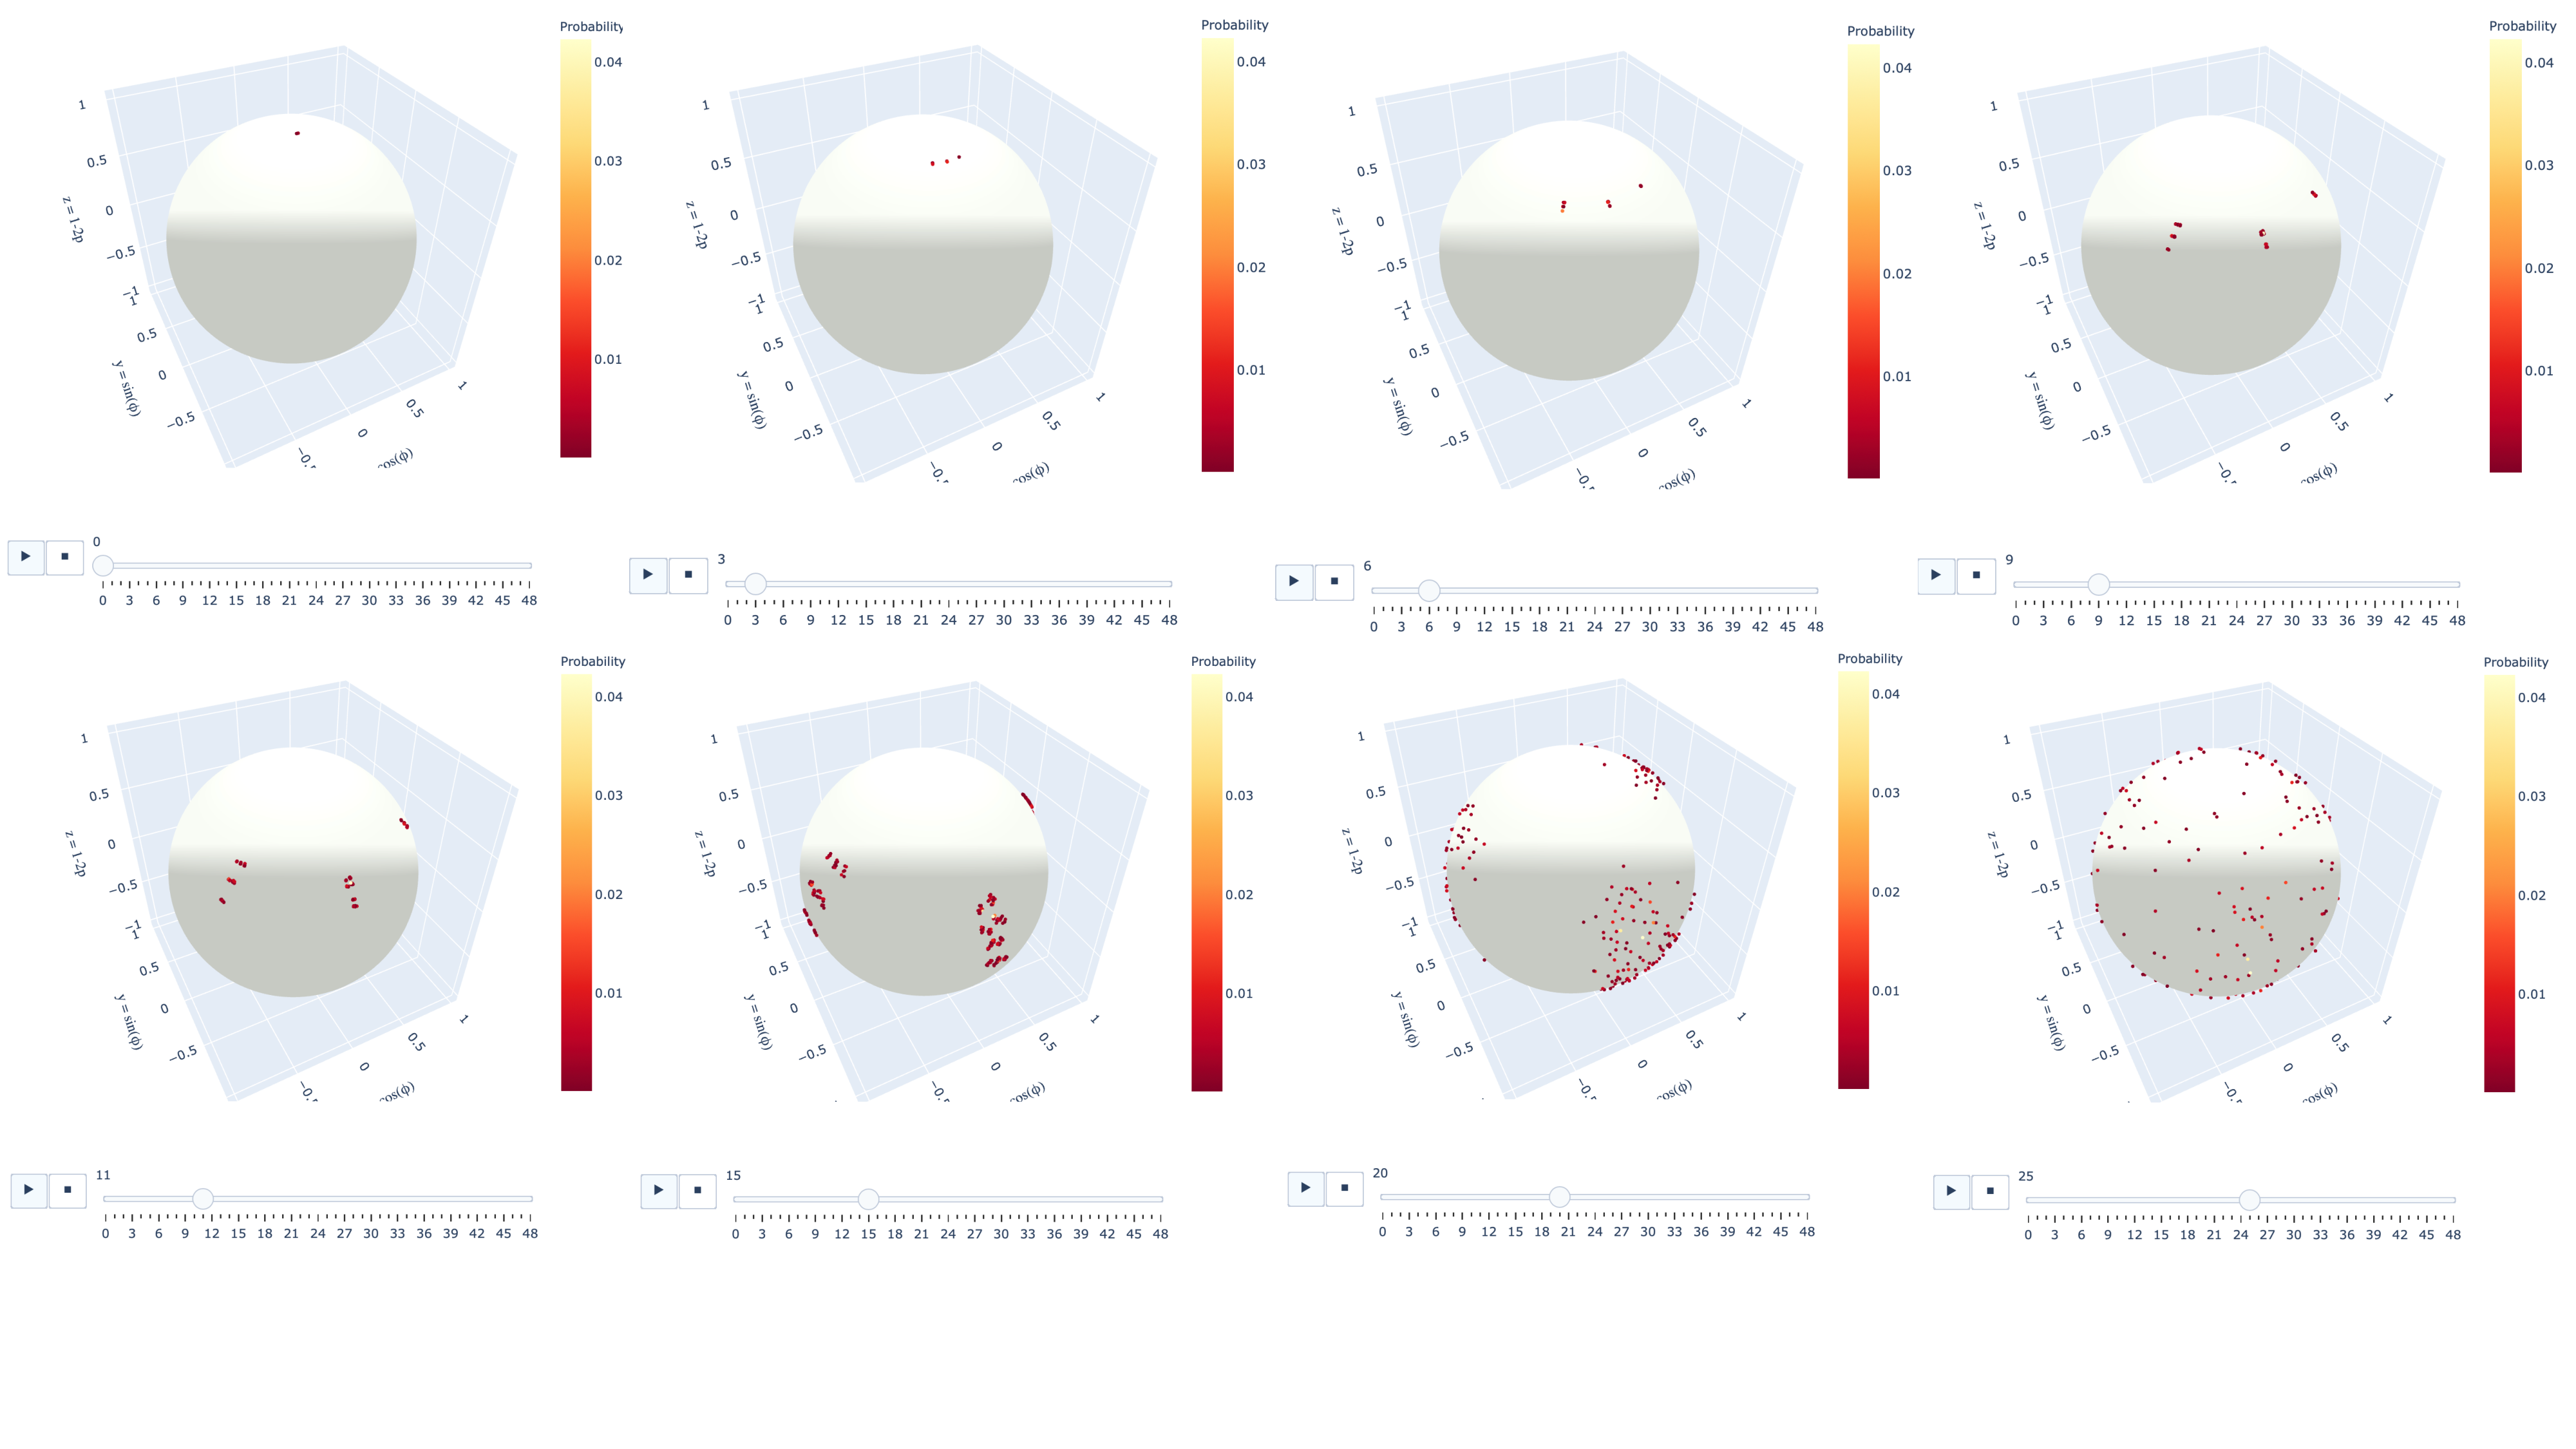
\includegraphics[width=.9\textwidth]{./img/DynamicsLong.pdf}
\caption{Evolution of the geometric quantum state of one qubit interacting with 
	nine others via an Ising model with transverse field, visualized on the surface of the Bloch
	sphere. Each point is $\Gamma_\alpha(t)$ and the color of the point encodes the probability
	$x_\alpha(t)$. Time increases left to right and top to bottom. Each point indicates 
	a possible state in which the system could be, and the color indicates the 
	probability of finding it in that state. The position of each point is determined 
	by the state of the environment and, indeed, there are $2^9$ points.
	}
\label{fig:gqs_dynamics}
\end{figure*}

\section{Information Transport: Continuity equation}
\label{sec:IT}

In the past section we have summarized previous results about GQM. In this 
section we build on them and, by bringing in the dynamics of the system, we derive 
a continuity equation which dictates how the geometric quantum state of a non-equilibrium 
open quantum system evolves, under very general assumptions. This is the fundamental 
kinetic equation that dictates how the information about the state of a quantum system 
changes as a result of its interaction with an environment. 
Throughout this section we will try to maintain a fairly general language, to emphasize
how the treatment applies to quantum systems under very general assumptions. However, 
for concrete examples we will always refer to the simple case of a qubit.



\subsection*{General treatment}
The following treatment pertains quantum systems which are finite-dimensional, and 
interact with finite-dimensional environments. Other than that, we continuity equation holds
for arbitrary quantum systems. 

Given an initial geometric quantum state, this is specified by two sets of quantities: $\left\{x_\alpha\right\}_{\alpha=0}^{d_E-1}$
and $\left\{ \Gamma_\alpha\right\}_{\alpha=0}^{d_E-1}$, which is a short-hand notation for 
$\Gamma_\alpha = Z(\ket{\chi_\alpha})$. The first one is a classical probability distribution
resulting from hypothetical measurements on the environment. For each of the $x_\alpha$
there is a corresponding pure state that the system inhabits: $\Gamma_\alpha \in \mathcal{P}(\mathcal{H}_S)$,
which corresponds to the ket $\ket{\chi_\alpha}$. Since these are points moving in a state space $\Gamma_\alpha(t)$,
we can think of them as particles on a classical phases space, which interact in a non-trivial
way. These are the ``carriers of information'', in the sense that each of these particles carries 
a probability mass $x_\alpha(t)$ that the system will be found on the state $\Gamma_\alpha(t)$.
A clarifying example of how the geometric quantum state of a qubit evolves when the system 
interacts with an environment is given in Figure \ref{fig:gqs_dynamics}. Since the total amount 
of information has to be preserved, $\mu_t(\PH) = \int_{\PH} q_t(Z) dV_{\mathrm{FS}} = \sum_\alpha x_\alpha(t) =1$,
the geometric quantum state $q_t(Z)$ must satisfy a continuity equation. Conceptually, this is 
the starting point of virtually all transport theories, which deal with quantities that are globally 
conserved, but that are moved around as a result of the underlying dynamics.


Thus, the dynamics of a geometric quantum state has two different terms, arising from the 
time-evolution of these two sets of quantities. By looking at Figure \ref{fig:gqs_dynamics}
we can see that there are two different ways in which the geometric quantum state changes 
in time. First, there is the color of each particle, which changes over time: $\dot{x}_\alpha \neq 0$. Second, there is
the pure movements of each point: $\dot{\Gamma}_\alpha \neq 0$. By summing each term over
all particles, and then summing the two terms, we get the following evolution equation for the geometric quantum state:
\begin{equation}
\frac{\partial q_t(Z)}{\partial t} = \sum_\alpha \dot{x}_\alpha \tilde{\delta}\left( Z- \Gamma_\alpha \right) - x_\alpha \widetilde{\delta}^{'}\left(Z - \Gamma_\alpha \right) \dot{\Gamma}_{\alpha}~.
\end{equation}
Here $\delta^{'}$ is the first distributional derivative of the dirac delta distribution. The second term in the
right-hand side can be written as a covariant divergence\footnote{With an arbitrary coordinate system we have $\mathrm{div} \vec{f} = \frac{1}{\sqrt{g}} \partial_\alpha \left(\sqrt{g} f^\alpha\right)$,
where $g = \vert \mathrm{det} g_{FS}\vert$ is the absolute value of the determinant of the metric which,
in our case, is the Fubini-Study metric.}, since every dipendence on the coordinate $Z$ is inside the delta distribution:
\begin{equation}
\sum_\alpha x_\alpha \widetilde{\delta}^{'}\left(Z - \Gamma_\alpha \right) \dot{\Gamma}_{\alpha} = (\nabla \cdot J_t)(Z)
\end{equation}
This allows us to identify the first functional term of the continuity equation, the \emph{flux of information} $J(t)$, which is 
a weighted average of the ``single-particle'' flux $J_\alpha(t)$:
\begin{subequations}\label{eq:flux}
\begin{align}
&J_\alpha(t) =  \widetilde{\delta}\left(Z - \Gamma_\alpha(t) \right) \dot{\Gamma}_{\alpha}(t)~,\\
&J(t) = \sum_\alpha x_\alpha(t)J_\alpha(t)~.
\end{align}
\end{subequations}
We now look at the first term in the right-hand: $\sum_\alpha \dot{x}_\alpha(t) \delta(Z-\Gamma_\alpha(t))$.
This is identified to be a source/sink term, which is independent on the underlying movement of
the points in the quantum state space. This identifies the second functional term of our continuity 
equation: \emph{sinks and sources of information} $\sigma_t(Z)$:
\begin{equation}
\sigma_t(Z) = \sum_{\alpha=0}^{d_E} \dot{x}_\alpha(t) \widetilde{\delta}\left(Z - \Gamma_\alpha(t) \right)~.\label{eq:sigma}
\end{equation}
Eventually, we obtain the following continuity equation for the geometric quantum state of a finite-dimensional
quantum system interacting with a finite-dimensional environment:
\begin{equation}
\frac{\partial q_t}{\partial t} + \nabla \cdot J_t = \sigma_t
\end{equation}
This is our first result. A crucial aspect here is that this theoretical framework allows us to talk about information 
as a physically localized (and overall conserved) quantity, which is carried around by points in quantum state space.
This is in analogy with the classical theories of information, which deal with properties of particles such as mass 
or charge, which are carried around by particles, represented as points wondering in a classical phase-space.
\begin{figure}[t!]
\centering
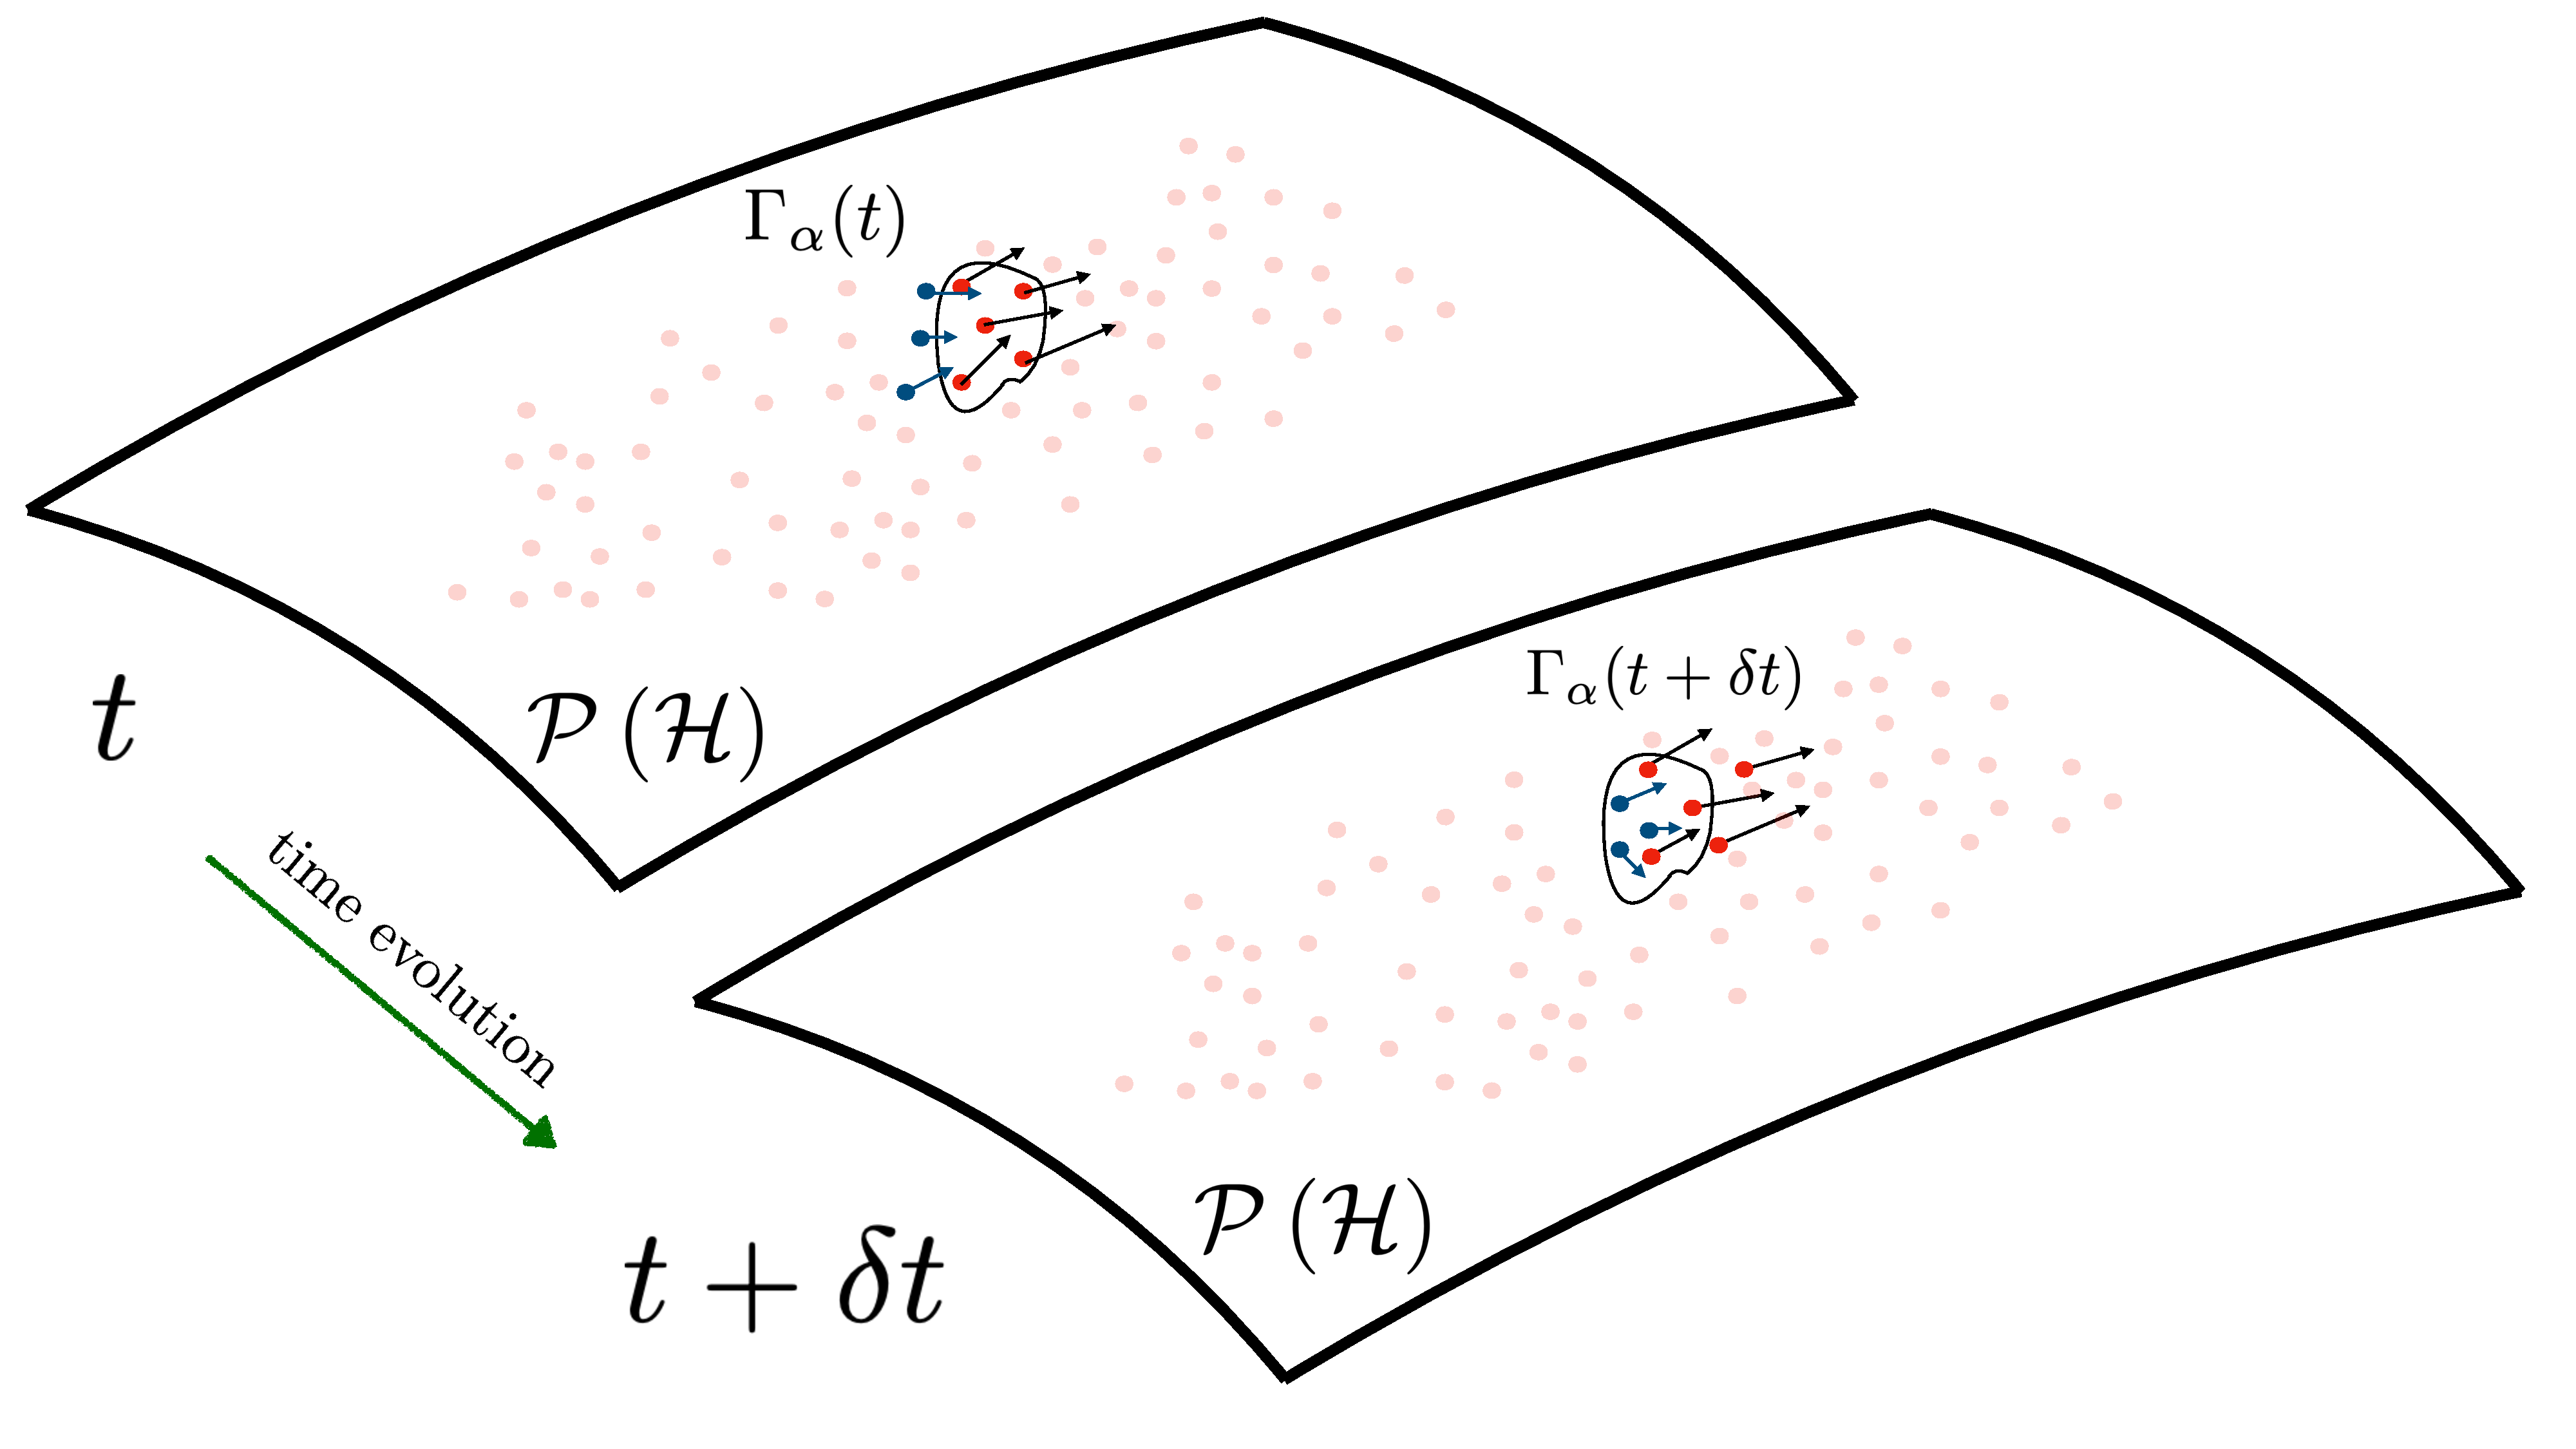
\includegraphics[width=.45\textwidth]{./img/Flux.pdf}
\caption{Kinetic interpretation of the flux $J$. If we look at a small region of the quantum state space, 
	due to the underlying dynamics we see that information is locally conserved in the sense that 
	there is a certain number of points which enters and leaves this region. As a result of this local
	process, probability is moved around and can concentrate in a certain region or get scrambled 
	across the quantum state space.
	}
\label{fig:flux_term}
\end{figure}

To reinforce this point, the physical interpretation of the flux $J_t$ and source/sink $\sigma_t$ term is essentially the 
same as in other transport theories. We now describe them explicitly, together with their kinetic interpretation, drawn
in Figures \ref{fig:flux_term} and \ref{fig:sigma_term}. First, $J_t$ is an information flux, in the proper sense of flux. As one can appreciate 
in Figure \ref{fig:flux_term}, this flux is associated to an overall conserved quantity, localized in its carriers $\Gamma_\alpha$, 
which move around and distribute it across the quantum state space. To emphasize this point we look at the simpler situation
in which $\dot{x}_\alpha = 0$. In this case, the information carried around by the points in state space is a constant
of motion ($x_\alpha(t)= x_\alpha(t_0)$). However, as the carriers move around, the information is still dispersed across
the quantum state space.

\begin{figure}[t!]
\centering
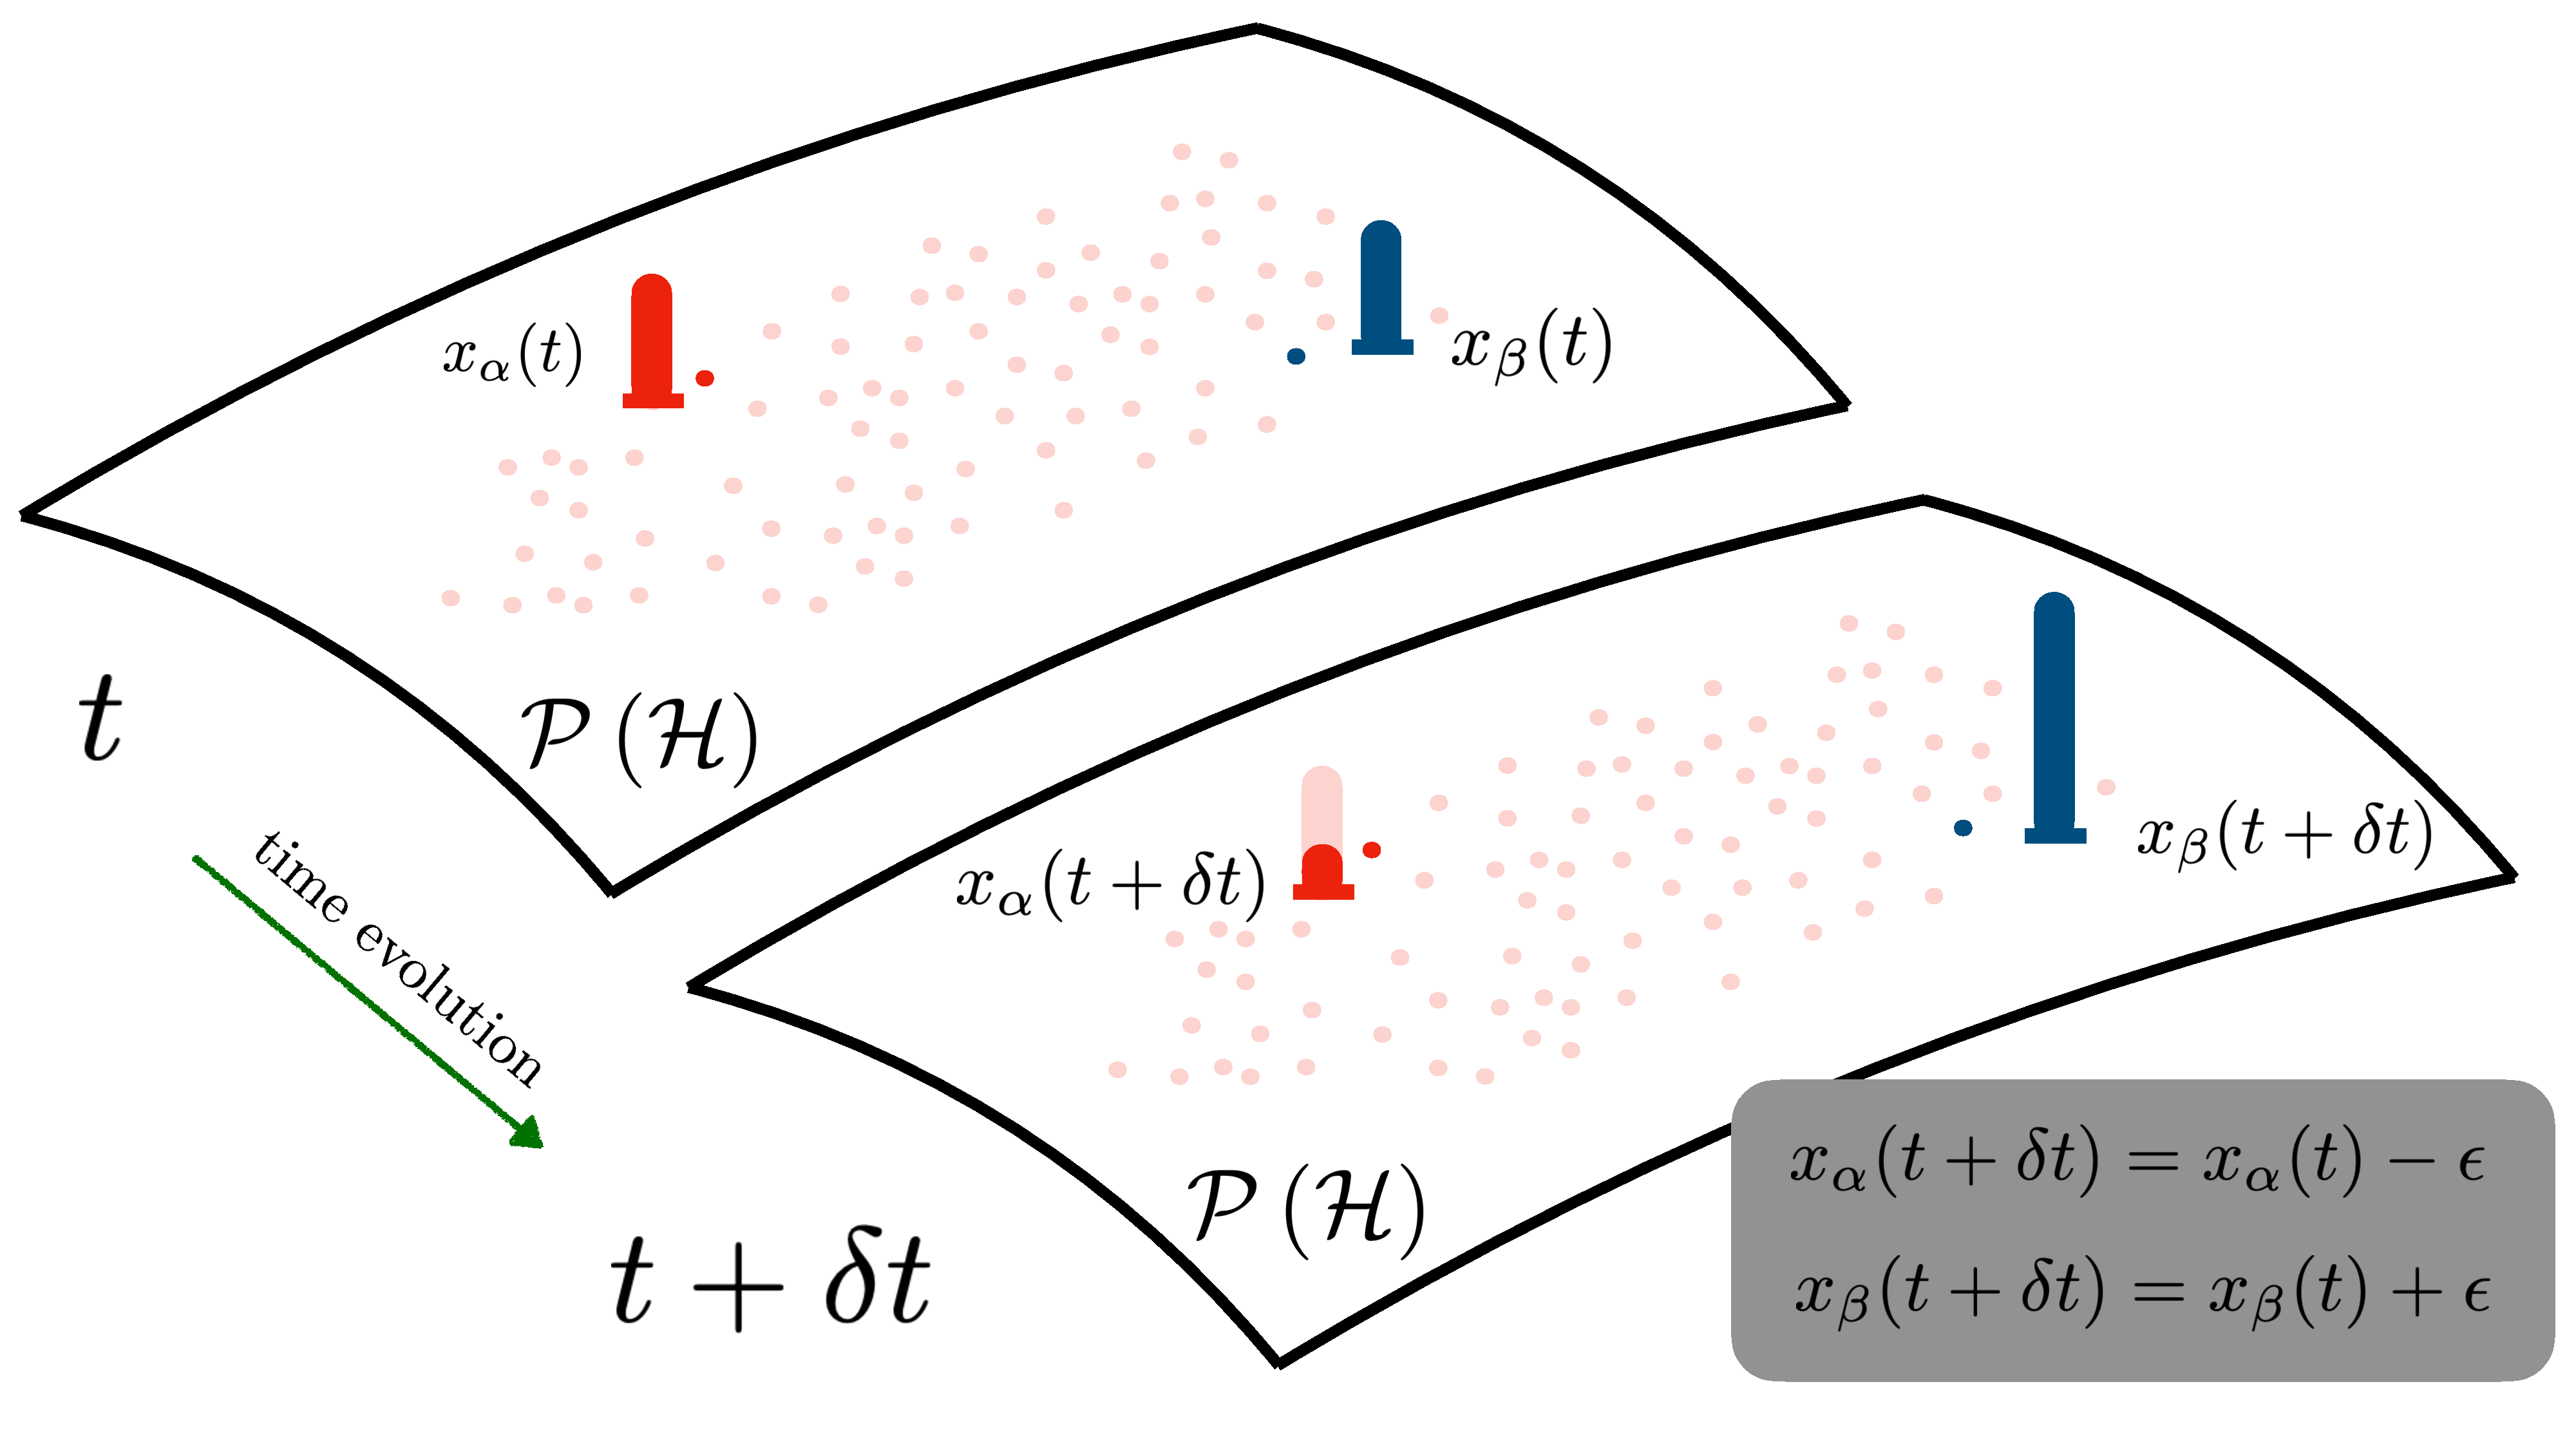
\includegraphics[width=.45\textwidth]{./img/Source.pdf}
\caption{Kinetic interpretation of the sink/source term $\sigma_t$. Even if the points do not move around
	the quantum state space $\dot{\Gamma}_\alpha=0$, the term $\sigma_t$ allows the exchange of information 
	between different regions. Note that this can be a non-local effect, as depicted above. In the example above
	we have two state $\Gamma_\alpha$ and $\Gamma_\beta$ fixed in time, but exchanging a certain amount of
	$\epsilon $probability, thus moving information from one region of the state space to another one: $x_\beta(t+\delta t) = x_\beta(t)+\epsilon$, $x_\alpha(t+\delta t) 
	= x_\alpha(t) - \epsilon$.
	}
\label{fig:sigma_term}
\end{figure}
Second, the term $\sigma_t$ is a proper source/sink term, with the usual interpretation. Indeed, we note that it
can not be written as a divergence term. To emphasize this point we look at the simpler dynamics in which the 
position of the points in $\PH$ does not change: $\dot{\Gamma}_\alpha = 0$. In this case the support of the 
distribution is fixed and the particles don't move $\Gamma_\alpha(t)=\Gamma_\alpha(t_0)$. However, even in 
this case there can still be a non-trivial dynamics, due to $\dot{x}_\alpha(t)\neq 0$. Moreover, as depicted
in Figure \ref{fig:sigma_term}, the time-evolution generated by this term is generally non-local in the quantum
state space. Thus, $\sigma_t$ possesses all the hallmarks of the standard sinks and sources terms in general 
transport theories: it is not associated with particles moving around the state space and it can not be rewritten 
as a divergence term.

\subsection*{Closed quantum systems}

What happens when the system is closed? Is there a specific form for the terms $J_t$ and $\sigma_t$?
Here we answer both these questions in a detailed manner. Since the evolution is Hamiltonian, we can 
use Hamilton's equations of motion to derive the evolution equation of $\mu_t$ or, equivalently, of $q_t(Z)$.
First, the sink/sources terms is trivially zero, as the evolution is Hamiltonian and preserves the local probabilities.
Second, starting from the definition of the flux in Eq.(\ref{eq:flux}), we can explicitly write the form of the flux $J_t$, 
using Hamilton's equations of motion. Writing $\Gamma_\alpha$ in canonical coordinates $(p_n(\Gamma_\alpha),\phi_n(\Gamma_\alpha))$, 
we have 
\begin{subequations}
\begin{align}
\dot{\Gamma}_\alpha & = \left\{\left( \dot{p}_n(\Gamma_\alpha), \dot{\phi}_n(\Gamma_\alpha)\right)\right\}_n\\
& = \left\{\frac{1}{\hbar}\left( \frac{\partial E}{\partial \phi_n}, -\frac{\partial E}{\partial p_n}  \right)\right\}_n = v_H(p_n,\phi_n)
\end{align}
\end{subequations}
Note how the right-hand side, which we called $v_H$ does not depend on the index $\alpha$ anymore: all 
the points evolve in the same way, following the same Hamiltonian flow. Inserting this into the definition of the flux 
we obtain that the flux is equal to the product between the distribution and the Hamiltonian velocity field $v_H$:
\begin{equation}
J_t(Z) = q_t(Z) v_H(Z)~,
\end{equation}
thus providing the following continuity equation:
\begin{equation}
\frac{\partial q_t}{\partial t} = - v_H \cdot \nabla q_t - q_t \, \nabla \cdot v_H
\end{equation}
This can be further simplified by noting that the Hamiltonian vector field is divergence free, $\nabla \cdot v_H = 0$, 
thanks to the fact that the Hessian of $E(p_n,\phi_n)$ is symmetric. Eventually, this leads us to the final form
of the continuity equation for a isolated quantum system:
\begin{equation}
\frac{\partial q_t}{\partial t} = - v_H \cdot \nabla q_t = -\left\{ q_t, E \right\}
\end{equation}

\paragraph*{Quantum Liouville's theorem.} As a further point of contact with the techniques of classical 
statistical mechanics, we now show that a generic Hamiltonian dynamics for the geometric quantum state 
satisfies Liouville's theorem \cite{Soto}. Indeed, by writing explicitly the total derivative of $q_t(Z)$ with 
respect to time we get 
\begin{equation}
\frac{d q}{d t} = \sum_\alpha \frac{\partial q_t}{\partial p_\alpha} \frac{dp_\alpha}{dt}+\frac{\partial q_t}{\partial \phi_\alpha} \frac{d\phi_\alpha}{dt} + \frac{\partial q_t}{\partial t}
\end{equation}
Inserting Hamilton's equations of motion (Eq. (\ref{eq:HAM_EOM})), and then using the continuity equation
\begin{align}
\frac{d q}{d t} &= \sum_\alpha \frac{\partial q_t}{\partial p_\alpha} \frac{dp_\alpha}{dt}+\frac{\partial q_t}{\partial \phi_\alpha} \frac{d\phi_\alpha}{dt} + \frac{\partial q_t}{\partial t}\nonumber \\
& = \left\{ q_t, E\right\} - \nabla \cdot q_t v_H = 0
\end{align}
This concludes the section about the general approach, and the treatment of isolated quantum systems.
We now turn to the more pertinent, and involved, case of an open quantum system.

\subsection*{Discussion}

\begin{itemize}
\item This kind of hamiltonian dynamics is more restrictive than a generic classical Hamiltonian dynamics: No chaos allowed, as the distance between points is constant.
\item Hence, we can concot Hamiltonian dynamics that violate this condition, possibly to give us quantum chaos.
\end{itemize}
%Upon unitary evolution the distribution remains 
%a Dirac delta, but 
%the point such state is concentrated on changes over time. For example, in the case of a 
%qubit we have coordinates $Z^0 = \sqrt{1-p}$ and $Z^1 = \sqrt{p}e^{i\phi}$. Hence we only 
%have a pair of independent canonically conjugated coordinates $(p,\phi)$. If the qubit is 
%isolated, with Hamiltonian $H = E_0 \ket{E_0}\bra{E_0} + E_1 \ket{E_1}\bra{E_1}$, we 
%can choose as a basis the Hamiltonian eigenstates and its evolution is simply written.
%Indeed, with this choice of coordinates we have $E(p,\phi) = E_0 + (E_1-E_0)p = E(p)$.
%Using Hamilton equations of motion (see Eq.\ref{eq:HAM_EOM}) we can see that $p$
%is preserved, $\dot{p} = \frac{1}{\hbar}\frac{\partial E}{\p \phi}=0$ and that $\phi$ is a cyclical
%coordinate $\dot{\phi} = - \frac{1}{\hbar} \frac{\partial E}{\partial p} = - \frac{E_0 - E_1}{\hbar}$, 
%giving $\phi(t) = \phi(t_0) - \frac{E_1-E_0}{\hbar}(t-t_0)$. This is easily generalized to
%the case of a generic Hilbert space, in which $p_\alpha$ are preserved and 
%$\phi_\alpha(t) = \phi_\alpha(t_0) - \frac{E_\alpha - E_0}{\hbar}(t-t_0)$. In a general coordinate
%system this means $q_t(Z) = \tilde{\delta}\left( Z - Z_t\right)$. 

%Unitary evolution do not spread information around the state space, but keep it localized, while
%moving around support of the distribution. 



\section{Kinetic theory of information transport in open quantum systems}
\label{sec:DYN}

As we move to analyze how open quantum systems move information around the
quantum state space, the goal of this section is to provide a microscopic approach
to the transport of information: a kinetic theory of how the information about the state
of a quantum system changes as a result of its interaction with a structured, non-thermal,
environment. Thus, the main outcome of this section is a concrete set of microscopic 
equations that determines the evolution of the geometric quantum state in a non-Hamiltonian 
setting.

Calling $H_S$ and $H_E$ the Hamiltonian operators of the system and environment, respectively, 
the total Hamiltonian of the joint system is $H = H_S + H_E + H_{\mathrm{int}}$. Since $H_{\mathrm{int}}$
is the interaction term between system and environment, we can always put it in the form
\begin{equation}
H_{\mathrm{int}} = \sum_{k} A^{(k)} \otimes B^{(k)}~,
\end{equation}
where $A^{(k)}$ and $B^{(k)}$ are operators with support on $\mathcal{H}_S$ and $\mathcal{H}_E$,
respectively. With a slight abuse of notation we will often conflate $A^{(k)}$ with $A^{(k)}\otimes \mathbb{I}_E$
and $B^{(k)}$ with $\mathbb{I}_S \otimes B^{(k)}$, where $\mathbb{I}_S$ and $\mathbb{I}_E$ are, respectively,
the identity operator on $\mathcal{H}_{S}$ and $\mathcal{H}_E$.



\section{Examples}
\label{sec:EXAMPLES}

\section{Conclusions}
\label{sec:FINAL}

Standard quantum mechanics' concept of state is the density matrix. However,
while density matrices provide a complete account of POVM statistics, they are
not in one-to-one correspondence with the ensembles that generated them. This
is a well-known fact that underlies the freedom in writing a decomposition of
the density matrix in terms of probabilities and pure states.  All such
decompositions yield the same POVM statistics, but they are not physically
equivalent since they are realized in physically different ways. The abiding
question then becomes: Which of these physically different ways exhibit
observable or, even perhaps, manipulable phenomena?

From a purification perspective \cite{Wilde2017}, the physical information
about an ensemble's realization can always be thought of as coming from a
larger system that is in a pure state. While the additional information about
how the ensemble is realized is not relevant for the measurement statistics on
our system, it does provide a much richer description. It preserves part (if
not all) of the structural information about how the system's POVM statistics
result from interactions with its surroundings.
 
Geometric quantum mechanics and its concept of geometric quantum state provide
a framework that allows retaining such information. This yields a richer
description of the system--one that goes beyond the system's POVM statistics, 
taking into account the physical manner in which an ensemble has been realized.
The geometric formalism's benefits emerge in at least two important cases:
(i) Hybrid continuous-discrete systems, e.g., electrons or other particles with
spin or other discrete degrees of freedom and (ii) the thermodynamic setting
of a system in contact with a large environment.

The geometric formalism directly handles the continuous nature of hybrid
systems and the large number of degrees of freedom in thermodynamics. And, it
does so in a fairly direct way. Thus, the geometric quantum state retains the 
structural information about how an ensemble is generated. While the 
two applications considered are similar, a crucial difference appears.

If we assume a finite environment, knowledge of the geometric quantum state of
our system is sufficient to recover the globally pure joint state of system and
environment. This does not occur for a hybrid discrete-continuous system, where
knowledge of the geometric quantum state does not allow inferring the phase
$\theta_0(\vec{x})$ of $f(\vec{x})$. Notably, fully recovering the overall pure
state, whose physical relevance can be argued on the ground of continuity with
the finite-dimensional case, effectively translates into a $U(1)$ gauge
principle on the overall system. The requirement that wave-functions differing 
from a local phase are physically equivalent---$\psi_s(\vec{x}) \sim
e^{i\varphi(\vec{x})}\psi_s(\vec{x})$---turns into a sufficient condition for
recovering the global pure state from the local geometric quantum state since, 
in this case, one can always choose $f(\vec{x}) \in \mathbb{R}$. Effectively, this is
the principle behind gauge symmetries and gauge theories. We must leave
exploring the connection between recovering the global pure state from a local
geometric quantum state and a gauge principle for a future investigation.

\paragraph*{Conclusion.}
Geometric quantum mechanics is an alternative to the standard vector-based
formalism. We introduced and then explored the concept of \emph{geometric
quantum state} $p(Z)$ as a probability distribution on the manifold of pure
states, inspired by the thermodynamic formalism of chaotic attractors from the
theory of dynamical systems or, more appropriately, its Sinai-Bowen-Ruelle
measures \cite{Eckmann1985}. This characterization accounts for the fact 
that singling out the density matrix as the sole descriptor of a quantum 
system's state entails ignoring how an ensemble is physically realized.
While this does not have observable consequences if one is restricted to POVM
statistics, in concrete situations the information about the ensemble
realization can be key to accurate modeling. Reference \cite{Anza20c} gives an
example. That said, the geometric setting is always sufficiently general
that density matrices are readily computed as quadratic averages from $p(Z)$
via Eq. (\ref{eq:densitymatrix}).

We explored the physical relevance of geometric quantum states via an open
quantum system in which a (finite) system under study is in contact with a
larger environment and their joint state is assumed to be pure. In this
thermodynamic setting, portions of the structural information about the joint
pure state is directly preserved in the geometric quantum state of the smaller
system under study. The result is a markedly richer picture of the system's
state---a picture that goes substantially beyond the density matrix and its
POVM statistics.

\section*{Acknowledgments}
\label{sec:acknowledgments}

F.A. thanks Marina Radulaski, Davide Pastorello, and Davide Girolami for
discussions on the geometric formalism of quantum mechanics. F.A. and J.P.C.
thank Dhurva Karkada for his help with the example and David Gier, Samuel
Loomis, and Ariadna Venegas-Li for helpful discussions and the Telluride
Science Research Center for its hospitality during visits.  This material is
based upon work supported by, or in part by, a Templeton World Charity
Foundation Power of Information Fellowship, FQXi Grant FQXi-RFP-IPW-1902, and
U.S. Army Research Laboratory and the U. S. Army Research Office under
contracts W911NF-13-1-0390 and W911NF-18-1-0028.

\bibliography{library}

\makeatletter
\newcommand{\manuallabel}[2]{\def\@currentlabel{#2}\label{#1}}
\makeatother

\clearpage
\appendix
\onecolumngrid

\pagestyle{empty}

\begin{center}
\large{Supplementary Materials}\\
\vspace{0.1in}
\emph{\ourTitle}\\
\vspace{0.1in}
{\small
Fabio Anza and James P. Crutchfield
}
\end{center}

\section{The Search for Quantum States}
\label{sm:QStates}

In those domains of the physical sciences that concern the organization and
evolution of systems, a common first task is to determine a system's distinct
configurations or \emph{effective states}. Ultimately, this turns on what
questions there are to answer. One goal is prediction---of properties or
behaviors. And, in this, quantum mechanics stands out as a particularly telling
arena in which to define effective states.

The very early history of its development can be construed partially as
attempts to answer this question, from de Broglie's \emph{phase-waves}
\cite{Brog25a} and Schrodinger's \emph{wave functions} \cite{Schr26a} to von
Neumann's \emph{statistical operators} in Refs. \cite{Neum27a} and \cite[Chap.
IV]{Neum32a}, later labeled \emph{density matrices} by Dirac
\cite{Dira29a,Dira30b,Dira31a}. And, these were paralleled by Heisenberg's
``operational'' \emph{matrix mechanics} that focused on experimentally
accessible observables and so avoided imputing internal, hidden structure
\cite{Heis25a}.

The abiding challenge is that effective states are almost always inferred
indirectly and through much trial and error. Quantum mechanics heightens the
challenge greatly due to its foundational axiom that the detailed, microscopic,
and fundamental degrees of freedom cannot be directly and completely measured
\emph{in principle}. The main text revisits this perennial question, What is a
quantum state?

\section{Theorem \ref{MainTheo}: Proof}
\label{sm:MainTheo}

This Appendix gives proves in detail Theorem \ref{MainTheo}.
Let's first restate its setup.

Consider a hybrid quantum system comprised of $N$ continuous degrees of freedom
and $M$ qudits that are the discrete ones. The entire system's Hilbert space
is:
\begin{align*}
\mathcal{H} = \mathcal{H}^c_N \otimes \mathcal{H}^d_M
  ~,
\end{align*}
where $\mathcal{H}_N^c$ hosts the continuous degrees of freedom and has
infinite dimension, while $\mathcal{H}^d_M$ hosts the discrete ones and has
dimension $d^M$. A basis for $\mathcal{H}_N^c$ is provided by
$\left\{\ket{\vec{x}}\right\}$, where $\vec{x} \in \mathcal{R} \subseteq
\mathbb{R}^N$ and a basis for $\mathcal{H}_M^d$ is
$\left\{\ket{s}\right\}_{s=0}^{d^M-1}$. Thus, a generic state is:
\begin{align}
\ket{\psi} = \int_{\mathcal{R}} d\vec{x} \sum_{s} \psi_s(\vec{x})\ket{\vec{x}} \ket{s}
  ~,\label{eq:first_step}
\end{align}
where $\vec{x}$ is a dimensionless counterpart of the physical continuous
degrees of freedom, achieved by multiplying its value by appropriate physical
quantities. So, the measure $d\vec{x}$ has no physical dimension. 


\emph{{\bf Theorem \ref{MainTheo}.}
Any state $\ket{\psi} \in \mathcal{H}$ can be written as:
\begin{align*}
\ket{\psi} = \int_{\mathcal{R}}d\vec{x} f(\vec{x}) \ket{x}\ket{q(\vec{x})}
  ~,
\end{align*}
where $f(\vec{x})$ is such that $\int_{\mathcal{R}}d\vec{x} |f(\vec{x})|^2 = 1$
and $\ket{q(\vec{x})}$ is a parametrized state of the discrete degrees of
freedom:
\begin{align*}
\ket{q(\vec{x})}
  = \sum_{s=0}^{d^M-1} \sqrt{p_s(\vec{x})} e^{i\phi_s(\vec{x})} \ket{s}
  ~,
\end{align*}
where $\left\{ p_s(\vec{x}),\phi_s(\vec{x})\right\}_s$ is a set of $2(d^M-1)$
real functions such that $\sum_{s=0}^{d^M-1} p_s(\vec{x}) = 1$,
$\phi_s(\vec{x}) \in [0,2\pi]$, and $\left\{\ket{s}\right\}_{s=0}^{d^M-1}$ is a
basis for $\mathcal{H}_M^d$.
}

\emph{Proof}: The proof is constructive. Given an arbitrary
$\left\{ \psi_s(\vec{x}) \right\}_s$, we can always find the set of functions
$f(\vec{x})$, $p_s(\vec{x})$, and $\phi_s(\vec{x})$. The converse holds
trivially: Given these functions one can always compute the $\left\{
\psi_s(\vec{x}) \right\}_s$. First, we define $\theta_s(\vec{x})$ as
the phase of $\psi_s(\vec{x})$:
\begin{align*}
\theta_s(\vec{x}) \in [0,2\pi[ \quad \mathrm{such \,\, that} \quad \psi_s(\vec{x}) = |\psi_s(\vec{x})| e^{i\theta_s(\vec{x})} 
  ~,
\end{align*}
and define the functions
\begin{align*}
\phi_s(\vec{x}) \coloneqq \theta_s(\vec{x}) - \theta_0(\vec{x})
  ~,
\end{align*}
Starting from Eq.(\ref{eq:first_step}) this gives

\begin{align*}
\ket{\psi} = \int_{\mathcal{R}} d\vec{x} \sum_{s} \psi_s(\vec{x})\ket{\vec{x}} \ket{s} = \int_{\mathcal{R}} d\vec{x} \sum_{s} \vert \psi_s(\vec{x}) \vert e^{i\theta_s(\vec{x})}\ket{\vec{x}} \ket{s} & =  \int_{\mathcal{R}} d\vec{x} \sum_{s} \vert \psi_s(\vec{x}) \vert e^{i\phi_s(\vec{x})+i\theta_0(\vec{x})}\ket{\vec{x}} \ket{s} \\ & = \int_{\mathcal{R}} d\vec{x} e^{i\theta_0(\vec{x})}\sum_{s} \vert \psi_s(\vec{x}) \vert e^{i\phi_s(\vec{x})}\ket{\vec{x}} \ket{s}
\end{align*}



We now define $f(\vec{x})$ and $p_s(\vec{x})$ as follows:
\begin{align*}
f(\vec{x}) & \coloneqq \sqrt{\sum_{s=0}^{d^M-1} \vert \psi_s(\vec{x}) \vert^2}
  \, e^{i \theta_0(\vec{x})} ~\text{and} \\
p_s(\vec{x}) & \coloneqq
  \frac{\vert \psi_s(\vec{x})\vert^2}{\sum_{l=0}^{d^M-1}\left\vert \psi_l(\vec{x})\right\vert^2}
  ~,
\end{align*}
It is easy to see how normalization of $|f(\vec{x})|^2$ and of $p_s(\vec{x})$ emerges from the definitions:
\begin{align*}
\int_{\mathcal{R}} d\vec{x} \left\vert f(\vec{x})\right\vert^2
  & = \int_{\mathcal{R}} d\vec{x}
  \sum_{s=0}^{d^M-1} \left\vert \psi_s(\vec{x}) \right\vert^2 \\
  & = 1 ~,\\
\sum_{s=0}^{d^M-1} p_s(\vec{x})
  & = \sum_{s=0}^{d^M-1}
  \frac{\vert \psi_s(\vec{x})\vert^2}{\sum_{l=0}^{d^M-1}\left\vert
  \psi_l(\vec{x})\right\vert^2} \\
  & = 1 ~,~\text{and} \\
\vert e^{i\phi_s(\vec{x})}\vert^2
  & = \frac{|\psi_s(\vec{s})|}{|\psi_s(\vec{x})|} \\
  & = 1
  ~.
\end{align*}
The latter gives $\phi_s(\vec{x}) \in [0,2\pi]$.

With these definitions we obtain:
\begin{align*}
e^{i\phi_s(\vec{x})} f(\vec{x}) \sqrt{p_s(\vec{x})}
  & = \sqrt{|\psi_s(\vec{x})|^2} e^{i\theta_s(\vec{x})} \\
  & = \psi_s(\vec{x})
  ~.
\end{align*}
This in turn gives the desired result:
\begin{align*}
\ket{\psi} & = \int_{\mathcal{R}} d\vec{x} \sum_{s} \psi_s(\vec{x})\ket{\vec{x}} \ket{s} \\
& = \int_{\mathcal{R}} d\vec{x} f(\vec{x}) \ket{\vec{x}}\sum_{s} e^{i\phi_s(\vec{x})}   \sqrt{p_s(\vec{x})}  \ket{s} \\
& = \int_{\mathcal{R}}d\vec{x} f(\vec{x}) \ket{x}\ket{q(\vec{x})}
  ~.
\end{align*}

%\bibliographystyleSM{apsr}
\bibliographySM{library}

\end{document}
